\section{AgentSquare Framework}

\begin{figure}[!t]
\begin{center}
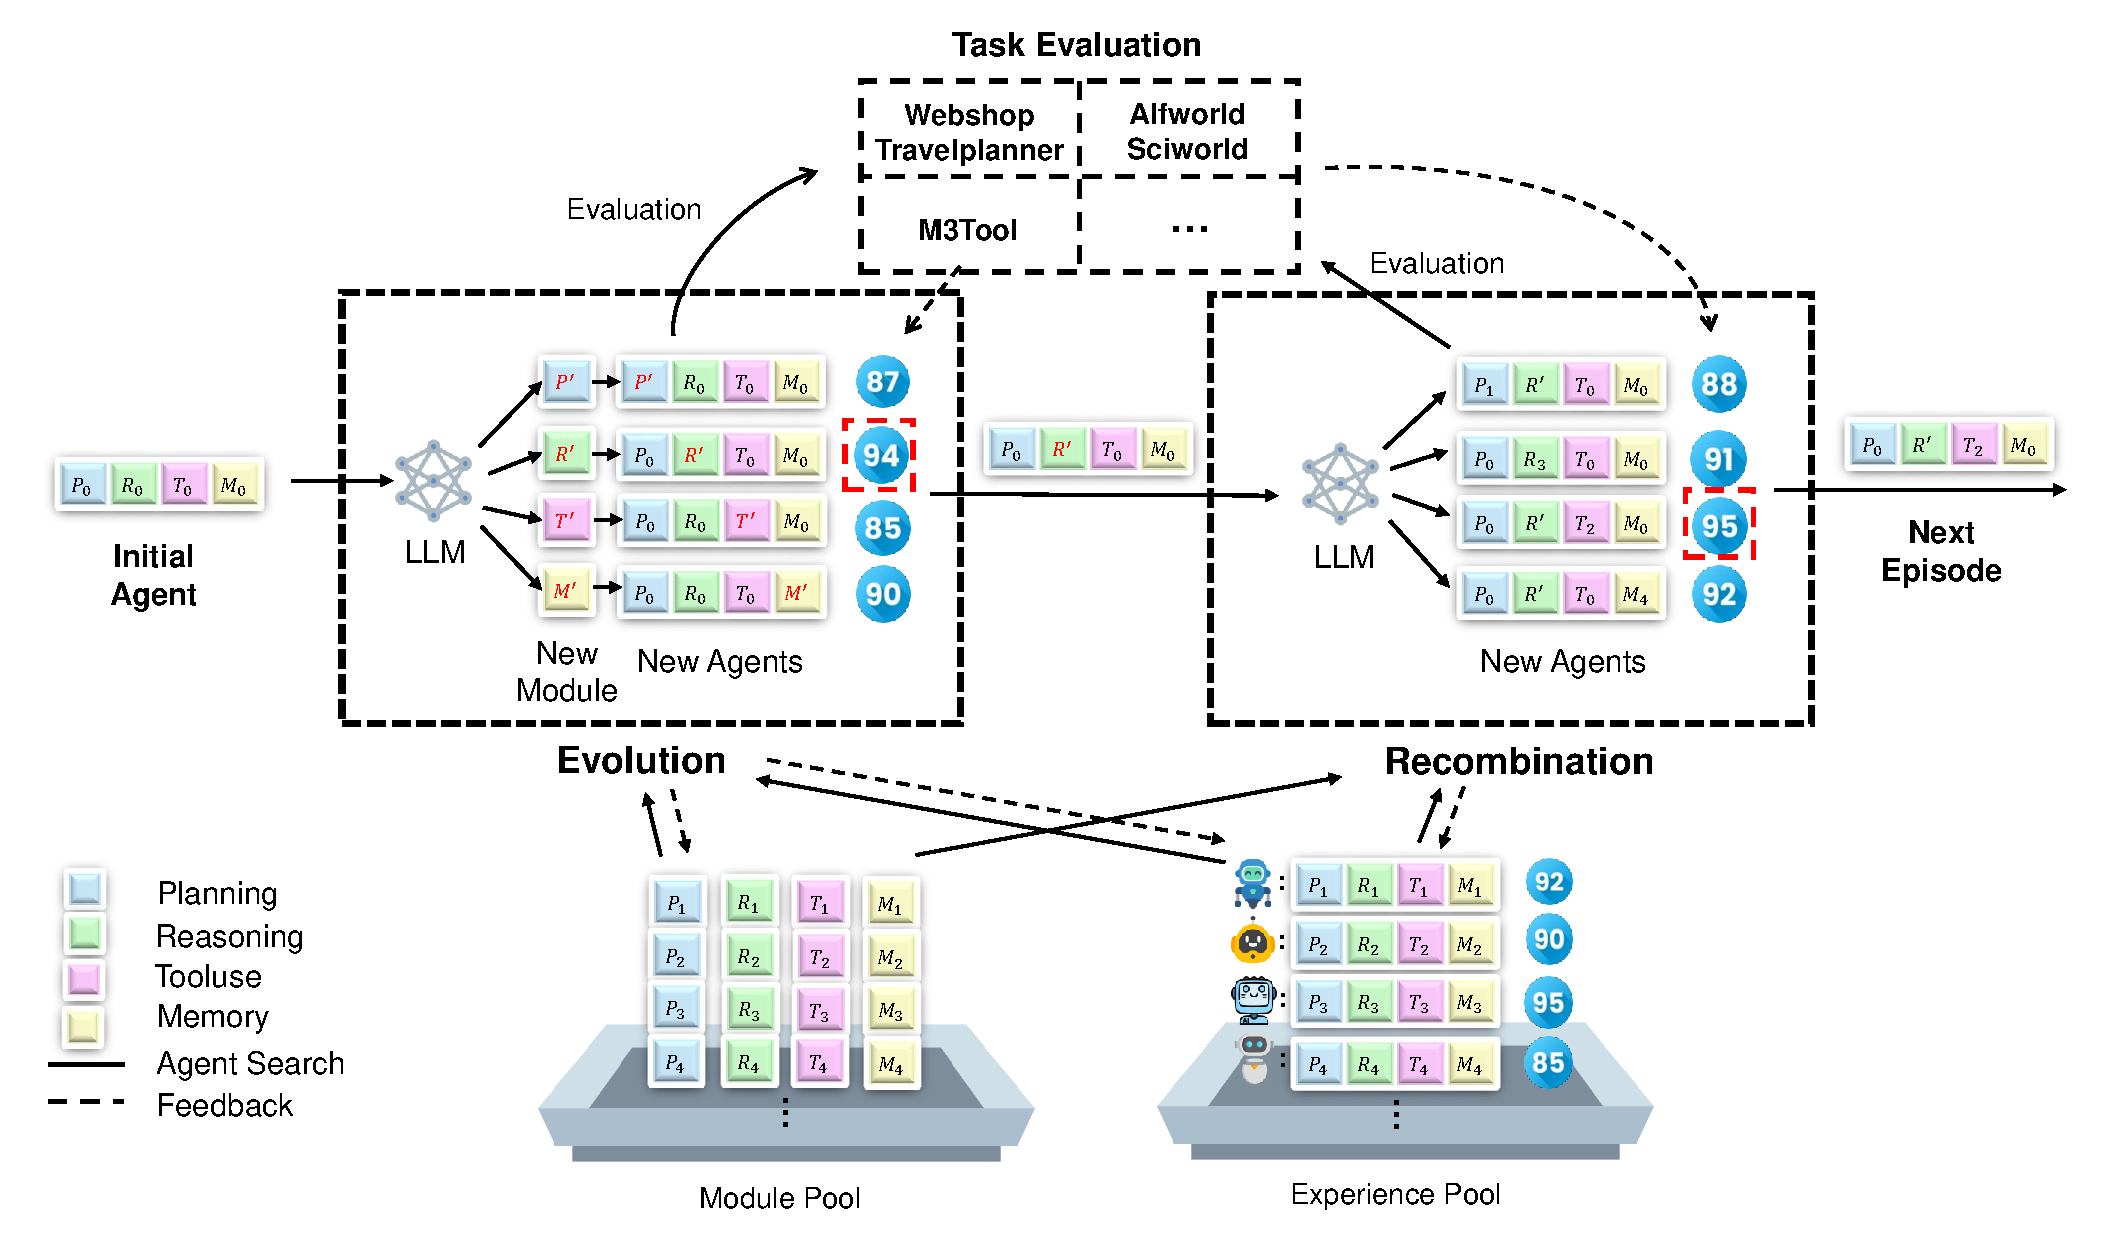
\includegraphics[width=12cm]{Figures/f3.pdf}
\caption{Overview of AgentSquare search framework. AgentSquare optimizes LLM agents through the mechanisms of module evolution and recombination. We further introduce a performance predictor that implements an in-
context surrogate model for efficient evaluation of novel agents.}
\label{framework}
\end{center}
\end{figure}
\subsection{Problem formulation of MoLAS}
In the proposed modular design space, an LLM agent $A$ can be instantiated with the combination of a planning module $P$, a reasoning module $R$, a tooluse module $T$ and a memory module $M$, denoted as $A = (P, R, T, M)$.
Given the task description $d$ and the set of all possible modules with standardized IO interface $\{\mathbb{P}, \mathbb{R}, \mathbb{T}, \mathbb{M}\}$.
We formulate an optimization problem for searching LLM agent architectures within the modular design space. 
The objective is to identify the optimal module combination in a solution space defined by a Cartesian product of four design dimensions to maximize agent performance.
Let the performance evaluation function of the task be ${Eval}_d(\cdot)$, where the specific metric varies in different tasks as discussed in Appendix~\ref{app:setup}. The optimization problem of MoLAS is defined as follows:
\begin{equation}
    \argmax\limits_{ P \in \mathbb{P}, R \in \mathbb{R}, T \in \mathbb{T}, M \in \mathbb{M}} {Eval}_d(P,R,T,M).
\end{equation}

\subsection{AgentSquare search algorithm}
Solving the optimization problem of MoLAS features three key challenges: (1) The search space, defined as the Cartesian product of four orthogonal modules, is vast and hard to explore;
(2) the module sets encompass any code with standard IO interfaces, making the module selection an open-ended problem; (3) the high costs of agent evaluation during the search process constrain the overall search scale.
To tackle these issues, we introduce AgentSquare, an automatic search framework to optimize LLM agents within the modular design space. 
Facing the vast search space of MoLAS, we propose \emph{module recombination} operation utilizing LLMs to strategically reason to identify more promising module combinations.
Such operation broadens the coverage of child samples, overcoming the limitations of prompt rewrite methods that explore only a restricted space.
However, only searching in the existing module combinations also narrows the search space, thus we propose \emph{module evolution} operation which employs an evolutionary meta-prompt to search new modules through code-level optimization.
This operation, combined with module recombination, enables the search of any module combination in the open-ended solution space.
Finally, to mitigate the high costs of frequent evaluations of searched agents, we design a \emph{performance predictor} as an in-context surrogate model for evaluating searched agents, significantly accelerating the search process and reducing real-valued costs.
% AgentSquare introduces three key designs for efficient agent optimization: \emph{module evolution}, which  \emph{module recombination}, which strategically switches certain modules with existing ones from standardized module pools, and \emph{performance predictor}, utilizing LLM to provide cost-efficient agent evaluation during search processes.

% In each search episode, AgentSquare optimizes an initial agent through alternating module evolution and recombination operations. 
% It starts with a module evolution phase programming new modules in code format.
% These newly created modules are individually integrated into the current agent, producing several child agents. 
% Each child agent is then evaluated, and the best-performing one is selected as the initial agent for the subsequent module recombination phase.
% During the recombination phase, AgentSquare utilizes an LLM to strategically replace certain modules with others from the standardized module pool.
% The generated agents are then evaluated, and the best one is selected as the initial agent in the next episode.
% Such search process is ended when it's unable to generate better agents or a predefined maximum number of search episodes $K$ is reached.
The overall framework of AgentSquare is illustrated in Figure~\ref{framework} and the algorithm is presented in Algorithm~\ref{alg}. 
Next, we detail the key components of the AgentSquare search process.

% \begin{algorithm}[t!] 
% % \SetAlgoNoLine 
% \caption{Algorithm of AgentSquare} 
% \label{alg}
% % \LinesNumbered 
% \KwIn{
% Initial agent $A_0$, targeted task descriptions $d$, maximum evolution episode $K$,  population size $N$ per evolution phase, standardized module pools $\{\mathbb{P}, \mathbb{R}, \mathbb{T}, \mathbb{M}\}$, experience pool $\mathbb{E}$ 
% }
% \KwOut{The evolved agent $A^*$}
% $t \leftarrow 1$ \tcp{Current search episode}
% $A_e^0 \leftarrow A_0$  \tcp{Initialization of the module evolution phase} 
% \While{$t \leq K$}{
% $\{A_e^1,A_e^2,...,A_e^N\} \leftarrow \pi_{\xi} (A_e^0, d, N, \mathbb{P}, \mathbb{R}, \mathbb{T}, \mathbb{M}, \mathbb{E})$ 
% \tcp{Module evolution}
% $A_r^0 \leftarrow \argmax\{{Eval}_d(A_e^0), {Eval}_d(A_e^1),...,{Eval}_d(A_e^N)\}$  \tcp{Select the best-performing generated agent} \\
% $\{A_r^1,A_r^2,...,A_r^N\} \leftarrow \pi_{\theta} (A_r^0, d, N, \mathbb{P}, \mathbb{R}, \mathbb{T}, \mathbb{M}, \mathbb{E})$ \tcp{Module recombination} \\
% $A_e^0 \leftarrow \argmax\{{Eval}_d(A_r^0), {Eval}_d(A_r^1),...,{Eval}_d(A_r^N)\}$ \tcp{Select the best-performing generated agent} \\
% $ t \leftarrow t+1$ 
% }

% $A^* \leftarrow A_e^0$ 

% \Return $A^*$
% \end{algorithm}

\subsection{Initialization}
Insights from existing AutoML studies indicate that a well-chosen initialization enhances warm-up and improves search efficiency by avoiding unpromising populations~\citep{so2019evolved,yuan2024evoagent}.
AgentSquare starts by initializing a global experience pool $\mathbb{E} = \{(P,R,T,M,v)|P_0 \in \mathbb{P}, R_0 \in \mathbb{R}, T_0 \in \mathbb{T}, M_0 \in \mathbb{M}\}$ to seed agents that are well-designed (as mentioned in Section 2) along with their real-valued performance $v$.
The module pools $\{\mathbb{P},\mathbb{R},\mathbb{T},\mathbb{M}\}$ are set to the standardized modules extracted from these seed agents.

\subsection{Module Recombination}
% Denote the initial agent in the module evolution phase as $A_e^0 = (P_0, R_0, T_0, M_0)$, where $P_0 \in \mathbb{P}, R_0 \in \mathbb{R}, T_0 \in \mathbb{T}, M_0 \in \mathbb{M}$. 
% represents the planning, reasoning, tooluse and memory module from corresponding standardized module pools.
Given the vast solution space of MoLAS, relying solely on prompt rewriting leads to a limited exploration confined to the neighbor of the initial state.
To expand the exploration space, we propose leveraging LLMs as a \emph{self-adaptive proposer}, which iteratively reason to identify promising module combinations with accumulated experience beyond the original agent configuration.
Denote the initial agent of the recombination phase as $A_r^0 = (P_0,R_0,T_0,M_0)$, where $P_0 \in \mathbb{P}, R_0 \in \mathbb{R}, T_0 \in \mathbb{T}, M_0 \in \mathbb{M}$.
The module combination proposer LLM $\pi_{\theta}$ incorporates targeted task description $d$, existing module pools $\{\mathbb{P}, \mathbb{R}, \mathbb{T}, \mathbb{M}\}$ and the performance experience of searched module combinations $\mathbb{E}$ to propose promising new agents $A_r$:
\begin{equation}
    A_r = \pi_{\theta}((P_0,R_0,T_0,M_0), d, N, \mathbb{P}, \mathbb{R}, \mathbb{T}, \mathbb{M}, \mathbb{E}).
\end{equation}

% The module evolution operation focuses on exploring novel modules to evolve agents, while the recombination operation aims to exploit existing modules to construct new agents.
% Denote the input agent of the recombination phase as $A_r^0 = (P^{'}_0,R^{'}_0,T^{'}_0,M^{'}_0)$, where $P^{'}_0 \in \mathbb{P}, R^{'}_0 \in \mathbb{R}, T^{'}_0 \in \mathbb{T}, M^{'}_0 \in \mathbb{M}$.
% The recombination operation leverages an LLM to strategically replace certain modules of the current agents with other existing modules, considering module profiles, targeted task descriptions, and performance experience of tested module combinations.
% The meta-prompt used for module recombination is presented in Figure~\ref{app:module-level1}.
Based on the initial agent configuration $A_r^0$, the LLM proposes $N$ offspring $\{A_r^1,A_r^2,...,A_r^N\}$ by replacing certain modules of $A_r^0$ with alternatives from the module pool. 
For instance, a possible solution could be $(P_0,R^{'},T_0,M_0)$, where $R^{'} \in \mathbb{R}$ is a different reasoning module selected from the module pool.
% Given the high cost of evaluating each generated agent in the task environment, here we introduce a cost-efficient agent performance predictor for agent evaluation.
% Specifically, we design a meta-prompt incorporating module profiles, targeted task descriptions, and performance history of previously tested agents for an LLM to predict the performance of newly generated agents.
% We have observed a strong correlation between the predicted and the agents' actual performance, showing the effectiveness of the performance predictor. 
% The results are presented in Figure X in the experimental section.
Then, the created $N$ new agents are evaluated with a performance predictor $\pi_p$ (detail in Seciton~\ref{section:pp}) and the best one goes to the next episode as initialization.

\subsection{Module Evolution}
As mentioned above, the solution space for each module type is open-ended, allowing any code with a standardized I/O interface. 
Consequently, searching only with module recombination narrows the solution space and limits the upper bound of agent performance.
To address this problem, we design a \emph{module evolution} operation with an evolutionary meta-prompt to search for new modules through program-level optimization.
This design is inspired by the iterative pipeline of FunSearch~\citep{romera2024mathematical}, which prompts LLMs to propose new solutions based on the target problem and performance feedback from existing solutions. 
Building on this concept, we introduce a module-programming LLM $\pi_{\xi}$ to conduct agent search in our modular design space by jointly modeling task descriptions, existing modules, and the performance of previously evaluated modules. Please note we reuse parts of the open-source code from ADAS~\citep{hu2024automated} to implement the optimization procedure.
Leveraging LLMs to search in the modular agent design space has several appealing advantages. 
Compared with the unconstrained design space of LLM agents, searching functional modules can produce a more focused and fruitful search space.
Additionally, integrating existing successful module designs with standard IO as in-context examples can better elicit the reflective reasoning abilities of LLMs to identify previous key designs to help propose innovative ones.
Denote the initial agent in the module evolution stage as $A_e^0 = (P^{'}_0,R^{'}_0,T^{'}_0,M^{'}_0)$, the module programmer LLM produces a population of child agents by evolving current modules of $A_e^0$.
Formally the module evolution operation is denoted as follows:
\begin{equation}
    A_e = \pi_{\xi}((P^{'}_0,R^{'}_0,T^{'}_0,M^{'}_0), d, N, \mathbb{P}, \mathbb{R}, \mathbb{T}, \mathbb{M}, \mathbb{E}).
\end{equation}

% \textbf{Targeted task description.}
% The first part is descriptions of the task assigned for the agent, including a high-level overview of the task and a specific task-solving trajectory demonstration.
% This information encourages the LLM to develop task-oriented modules.
% For instance, a sophisticated planning module is crucial for embodied tasks like ALFWorld, where multi-step action sequences are needed. 
% In contrast, it is less critical for tool-use tasks, which often require single-step decisions.

% \textbf{Existing module codes.}
% We structurally organize the codes of existing modules extracted from existing literature with corresponding design insights and integrate them into the meta-prompt.
% These information serves as the foundation for the LLM to program new modules.

% \textbf{Past module performance.}
% Another key information for better module discovery is the performance experience of existing modules.
% We present the performance of a series of agents selected from the experience pool $\mathbb{E} = \{(P,R,T,M,v)|P_0 \in \mathbb{P}, R_0 \in \mathbb{R}, T_0 \in \mathbb{T}, M_0 \in \mathbb{M}\}$, where $v$ denotes the agent performance.
% The selected agents differ along a single design dimension, which can serve as indicators for specific modules. 
% Incorporating this into the meta-prompt enables the LLM to recognize performance patterns across modules, thereby guiding it to leverage high-performing solutions and construct superior ones.
The created new modules are appended to the standardized module pools $\{\mathbb{P}, \mathbb{R}, \mathbb{T}, \mathbb{M}\}$ and each module is used to individually mutate the initial agent, resulting in $N$ child agents $\{A_e^1,A_e^2,...,A_e^N\}$.
For example, $(P^*, R_0, T_0, M_0)$ represents a solution where the planning module is mutated into a new variant $P^*$.
These child agents are then real-tested and updated to the historical experience pool $\mathbb{E}$. 
The best-performing one is selected as the initial agent for the subsequent recombination phase.

\subsection{Performance Predictor} \label{section:pp}
The last challenge in automatic agent search is the high API cost incurred during the evaluation of each candidate agent.
Many agent tasks require multiple steps and involve substantial input and output tokens, leading to prohibitive evaluation costs.
For instance, evaluating a simple CoT agent based on GPT-4o in ALFWorld~\citep{shridhar2021alfworld} requires around \$60, making the agent search economically unsustainable at scale.
To tackle this issue, we propose incorporating an additional LLM $\pi_p$ as a performance predictor to serve as an in-context surrogate model for novel agent evaluation, enabling the exclusion of unpromising candidates and significantly accelerating the search process.
Compared to real environment evaluation, such an in-context surrogate model requires significantly fewer tokens, making it more cost-efficient and supporting larger-scale searches.
Similar approaches have been effectively applied in neural architecture search (NAS), where LLMs are leveraged to evaluate the performance of generated network architectures ~\citep{jawahar2023llm,chen2024evoprompting}.
% The meta prompt of the performance predictor is shown in Figure~\ref{app:pp-prompt}.

During the search process, newly created agents from module evolution are still tested in the real task environment because these new modules never appear in the experience pool, and it is unsuitable to use the performance predictor to provide predictions.
During the module recombination operation, the newly proposed agents are evaluated by the performance predictor, which leverages in-context reasoning based on past agent combination performance to provide efficient performance prediction.  
Here, given a newly searched agent $A'$, the performance predictor $\pi_p$ thoroughly considers task descriptions $d$, module profiles and in-context performance examples of previously tested agents $\mathbb{E}$ to score novel agents:
\begin{equation}
    v' = \pi_p(A', d, \mathbb{P}, \mathbb{R}, \mathbb{T}, \mathbb{M}, \mathbb{E}),
\end{equation}
where $v'$ is the predicted performance of the evaluated agent.
Empirical results demonstrate that the predicted performance of agents closely matches their actual performance, verifying the effectiveness of the proposed performance predictor, which is detailed in Section~\ref{technical}.


